% Use class option [extendedabs] to prepare the 1-page extended abstract.
\documentclass[extendedabs]{bmvc2k}

% For the final submission, comment out the bmvcreviewcopy so that
% author names etc appear.
%\bmvcreviewcopy{1234}

% Enter a shortened version of the title as a running header.
% For two authors, enter both surnames, separated by commas.  For
% more than two authors, the first author's name followed by
% \bmvaEtAl will produce the correct output (uppercase author name,
% lowercase etal).  This will not appear in the extended abstract
\runninghead{Claus, Fitzgibbon}{Plumbline Constraint for the RF Model}
% \runninghead{Claus \bmvaEtAl}{Plumbline Constraint for the RF Model}

% Document starts here
\begin{document}

\title{Report: Computer Vision (CSL462) Assignment-1}

% Notice that there is a reasonable amount of whitespace around the
% author names.  There should be no reason to compress this for the
% online proceedings as the page limit is counted from the bottom
% of the author list.
%
% While it may be tempting to compress this for the extended
% abstract, please resist the temptation to overdo it.  This 1-page
% abstract is currently three pages in normal BMVC style, which
% should be plenty of space for your key idea, figure, and
% references.
\addauthor{Chirag Khurana}{2016csb1037@iitrpr.ac.in}{1}

\addinstitution{
Department of Computer Science,\\
Indian Institute of Technology Ropar}
\maketitle

% Extended abstract begins here.  In a one-page document, there is
% little need for section headers, but you may use \section etc if you
% wish.

\section{Objective}
To adaptive blur on image based on edge/color/template information. Foreground should be highlighted and the background should be blurred.

\section{Second Order Edge Detection}
The \textbf{Marr-Hildreth algorithm} is applied for edge detection. It is a method of detecting edges in digital images, that is, continuous curves where there are strong and rapid variations in image brightness. The Marr-Hildreth edge detection method is simple and operates by convolving the image first with the Gaussian filter and then the Laplacian filter.Then, zero crossings are detected in the filtered result to obtain the edges. Outputs images are shown in Figure-2.\\
\\
Gaussian Operator:
\begin{equation}
    g(x,y)=\frac{1}{{2\pi\sigma^2  }}e^{{{ - ({x}^2 +{y}^2)}/{2\sigma ^2 }}}
\end{equation}
Laplacian Operator:
\begin{equation}
\begin{bmatrix}
0&1&0\\
1&-4&1\\
0&1&0
\end{bmatrix}
\end{equation}

\begin{figure}[t]
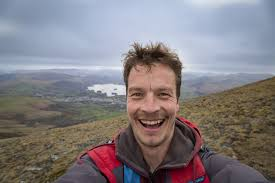
\includegraphics[width=\linewidth]{temp1.jpg}
\caption{
Orignal Image For Edge Detection}
\vspace{-2mm}
\end{figure}


\begin{figure}[t]
\includegraphics[width=\linewidth]{temp2.jpg}
\caption{
Edge detection a) With Edge Magnitude b) Binary Image}
\vspace{-2mm}
\end{figure}

\section{Adaptive Blur Computation}
Foreground and background are distinguished based on the local average edge density.
Following Steps are used to blur the image:
\begin{enumerate}
    \item Edge detection done using above given method with $\sigma=0.2$ and output is taken with edge magnitudes.
    \item Average of pixel values calculated.
    \item Then image is made binary using:
    \[
    \begin{cases}
    1&\text{if pixel value >= 3xAverage}\\
    0&\text{otherwise}\\
    \end{cases}
    \]
    Image shown in Figure 3, which almost distinguished foreground and background.
    \item Let MxN be size of the image. Now, a window of size of M/10xN/10 is moved on the image and window is blurred using the $\sigma$ which is calculated using the \textbf{Extract Statistics} function which is discussed in the next section.
    \item Then, finally background blurred image is created.\\
    \\Output Images are shown in Figure-4,5
\end{enumerate}



\begin{figure}[t]
\includegraphics[width=\linewidth]{edgec.jpg}
\caption{
Adaptive Blur Step-3 Output}
\vspace{-2mm}
\end{figure}

\begin{figure}[t]
\includegraphics[width=\linewidth]{1.jpg}
\caption{
Adaptive Blur Output Image-1}
\vspace{-2mm}
\end{figure}



\section{Extract Statistics}
This function calculates $\sigma$ for a image portion(window) (say I1) based on binary edge detected image (say I) of Adaptive Blur Step-3. Let A be the average pixel value of the I and A1 be the average pixel value of the I1.\\Then,
 \[ \sigma=
    \begin{cases}
    \text{min(5,(min(4,A/2)-A1)}&\text{if A1<min(4,A/2)}\\
    2&\text{if A1<=A/2}\\
    0&\text{otherwise}\\
    \end{cases}
    \]
    
\section{References}
1. Marr-Hildreth Algorithm-Wikipedia\\
2. Gauss Filter-Wikipedia\\
3. Image Source-Google

\begin{figure}[t]
\includegraphics[width=\linewidth]{2.jpg}
\caption{
Adaptive Blur Output Image-2}
\vspace{-2mm}
\end{figure}

\begin{figure}[t]
\includegraphics[width=\linewidth]{3.jpg}
\caption{
Adaptive Blur Output Image-3}
\vspace{-2mm}
\end{figure}

\end{document}

